%\chapter{Desenvolvimento do Jogo}
\chapter{Resultados Parciais}
\label{chap:des}

Neste capítulo é apresentado como se deu a execução da metodologia adotada neste trabalho e já alguns resultados parciais. Os resultados parciais são os documentos de design apresentando a ideação do jogo e a definição de aspectos técnicos para construção de um software.

\section{Ciclo de vida do jogo}

Como apresentado no Capítulo \ref{chap:Metodo}, o desenvolvimento do jogo PersonaDesignGame inicia-se a partir de uma revisão da literatura e definição do escopo. Esse processo segue se apoiando no \textit{Playcentric Design Process} juntamente com algumas diretrizes da Engenharia de software. Na revisão da literatura, além da base de conhecimento para realização do projeto, foi possível levantar alguns requisitos a partir da identificação dos trabalhos sobre jogos em IHC mencionados no Referencial Teórico, Capítulo \ref{chap:ref}, Seção \ref{sec:trab_cor}. 

Na etapa de definição de escopo foi elaborado um \textit{survey}, no qual foi desenvolvido e aplicado um questionário de pesquisa, que teve como objetivo identificar o público-alvo e elicitar mais alguns requisitos. O relatório do \textit{survey} é descrito no Apêndice \ref{ap:questionario} assim como o próprio questionário. Para finalizar essa etapa e fechar o escopo foram elaboradas personas, estas guiaram a definição, especificação e validação dos requisitos identificados.

O elenco de personas criado também participou de todo o processo de design ao longo do projeto. Como persona primária, o arquétipo alvo do projeto, temos Victor Matheus Farias; como persona secundária temos o Afonso de Souza Queiroz; como persona suplementar temos a Natália Figueiredo; e por fim temos a anti-persona Rafael Medeiros. Todas elas estão detalhadas no Apêndice \ref{ap:persona}, assim como o processo de sua construção.

{\color{textmodified}
A partir das personas definidas, foram elaboradas a ideia base do jogo, definidos os requisitos funcionais, não funcionais e as metas de experiência do jogador, e elaborado uma primeira versão do protótipo de papel (Apêndice \ref{ap:proto_papel}). Isso tudo está descrito no Game Design Document, Seção \ref{sec:gdd} e no Technical Design Document, Seção \ref{sec:tdd}.
}

{\color{textadded}

Com a primeira versão do protótipo de papel, foram realizados dois ciclos de validação (Apêncide \ref{ap:proto_papel}). Para isso foi utilizado o planejamento das atividades citadas por \citeauthor{barbosa_silva} \citeyear{barbosa_silva}, no qual foram executadas as atividades de preparação, coleta de dados e interpretação, consolidação e relato de resultados (Tabela \ref{tab:aval-prot-papel}). Durante essa validação, foram detalhados e adicionados novos requisitos para o projeto (Subseção \ref{ssec:requisitos}).

Após a realização da validação dos requisitos através do protótipo de papel, foi definida a arquitetura do software, Seção \ref{sec:arq}. A arquitetura é composta de dois microserviços e um front-end (Figura \ref{Fig:diagrama_arquitetura.png}), utilizando de tecnologias como \citeauthor{reactjs}, \citeauthor{nodejs} e \citeauthor{mysql}.

Com toda a arquitetura do software definida, foram criadas algumas políticas importantes para o início do desenvolvimento como políticas de \textit{issues}, políticas de \textit{branch} e políticas de \textit{commits} (Seção \ref{sec:gces}). Também foi definida a ferramenta \textit{Docker} para a configuração do ambiente de desenvolvimento (Subseção \ref{ssec:config_amb}) e a pipeline seguida para a integração contínua e entrega contínua do software (Subseção \ref{ssec:ci_cd}).

A seguir é apresentado o documento de design do jogo, na qual são definidos e apresentados os principais conceitos do jogo PersonaDesignGame.

}

\section{Game Design Document}
\label{sec:gdd}
Nesta seção é apresentado o GDD, documento no qual estão especificados as características gerais do jogo, \textit{gameplay}, mecânica e fluxo do jogo, regras e os seus elementos. Este artefato é evolutivo, sendo incrementado e sofrendo alterações ao longo do projeto.

\subsection{Características Gerais}

{\color{textmodified}
O jogo elaborado neste trabalho é o PersonaDesignGame, um jogo educacional sobre personas. Este é classificado como um jogo de gênero educacional de perguntas e respostas. Trata-se de um jogo 2D, com uma perspectiva em primeira pessoa, no qual o modo de jogo é \textit{single player}.
}

O PersonaDesignGame tem como seus jogadores-alvo, alunos de graduação e pós-graduação em cursos da área de Ciência da Computação. Neste jogo o estudante irá aprender o conteúdo sobre a técnica de personas, exercitá-lo e por fim ter um exemplo prático de como se construir uma persona.

\subsection{Gameplay}

O objetivo do jogo é ensinar o conteúdo sobre personas enquanto o usuário joga. Para isso o jogo segue uma mecânica de perguntas e respostas. O usuário progride no jogo ao responder às perguntas seguindo o fluxo apresentado na Figura \ref{Fig:game_flow.png}.

\begin{figure}[htbp]
	\centering
		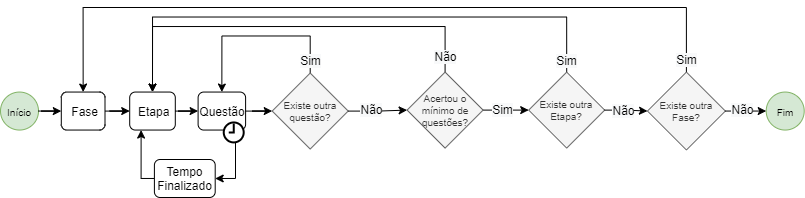
\includegraphics[keepaspectratio=true,scale=0.56]{figuras/game_flow.png}
		\caption{\textcolor{textmodified}{Fluxo da Partida do Jogo - Próprios Autores}}
	\label{Fig:game_flow.png}
\end{figure}

\newpage

{\color{textmodified}
O jogador inicia a partida selecionando a etapa de uma fase que esteja liberada. Iniciada a partida, o jogador recebe um trecho do conteúdo sobre personas referente ao tema desta etapa da fase. Em seguida o cronômetro começa a contar e é apresentada uma questão. 

Ao responder a questão o jogador então pode receber um feedback positivo (resposta certa) ou negativo (resposta errada). O jogador prossegue respondendo enquanto houverem questões na etapa e enquanto o tempo não acabar. Caso ele finalize a etapa dentro do tempo e com o mínimo de questões respondidas corretamente, o jogador libera a próxima etapa. Caso não cumpra estas regras o jogador deve repetir a etapa. 

O jogador segue esse ciclo até finalizar todas as etapas em todas as fases. As questões são agrupadas por temas de conteúdo, compondo as fases, e cada fase têm grupos menores de questões, as etapas. Ao todo são duas fases que contemplam os aspectos gerais sobres as personas e sobre a construção de personas, como é descrito a seguir:
}

\begin{itemize}
    \item \textbf{Fase 1:}
    
    \textbf{Tema:} Aspectos Gerais sobre Pesonas.
    
    \textbf{Tipo de Questão:} Verdadeiro ou Falso; Múltipla Escolha.
    
    \item  \textbf{Fase 2:} 
    
    \textbf{Tema:} Aspectos da Construção Pesonas.
    
    \textbf{Tipo de Questão:} Verdadeiro ou Falso; Múltipla Escolha.
    
\end{itemize}

{\color{textmodified}
Ao longo das questões algumas dicas são habilitadas para que o jogador possa relembrar de algum termo sem precisar voltar ao conteúdo apresentado anteriormente. Durante a resolução das questões, \textit{cards} de característica de personas podem ser coletados como recompensa, e além disso o jogador pode cumprir desafios propostos e ser recompensado com medalhas ao longo do jogo. A seguir são apresentados mais detalhes sobre estes elementos presentes no jogo.
}

\subsection{Elementos do Jogo}

{\color{textmodified}
O jogo PersonaDesignGame possui três ambientes. O menu inicial é resposável por dar acesso a estes ambientes. O primeiro ambiente é a própria partida do jogo, na qual o jogador pode iniciar a resolução das questões. Existe também o ambiente de resumos, no qual o jogador tem acesso ao conteúdo sobre as personas. Por fim no ambiente de recompensas são apresentadas as medalhas obtidas e as personas com seus respectivos \textit{cards}.
}

{\color{textadded}
As medalhas são recompensas obtidas ao se completar desafios durante uma partida. Estes desafios variam entre as seguintes categorias: tempo de resposta, combo de acerto e combo de etapas completas. Existem três tipos de medalhas: de ouro, prata e bronze. A seguir é listado os requisitos para a obtenção das medalhas em cada uma das categorias.

\begin{itemize}
    \item Tempo de resposta
    \begin{itemize}
        \item \textbf{Medalha de Ouro} - Completar etapa com até 30\% do tempo da fase.
        \item \textbf{Medalha de Prata} - Completar etapa com 31\% até 60\% do tempo da fase.
        \item \textbf{Medalha de Bronze} - Completar etapa com 61\% até 80\% do tempo da fase.
    \end{itemize}
    \item Combo de acerto
    \begin{itemize}
        \item \textbf{Medalha de Ouro} - Acertar 15 questões seguidas.
        \item \textbf{Medalha de Prata} - Acertar 10 questões seguidas.
        \item \textbf{Medalha de Bronze} - Acertar 5 questões seguidas.
    \end{itemize}
    \item Combo de etapas
    \begin{itemize}
        \item \textbf{Medalha de Ouro} - Concluir 5 etapas seguidas sem falhar.
        \item \textbf{Medalha de Prata} - Concluir 3 etapas seguidas sem falhar.
        \item \textbf{Medalha de Bronze} - Concluir 2 etapas seguidas sem falhar.
    \end{itemize}
\end{itemize}

}

{\color{textmodified}
Já as recompensas em \textit{cards} estão relacionados às características de alguns exemplos de personas. Os \textit{cards} recompensa são os seguintes: identidade, objetivos, habilidades, tarefas, relacionamento, requisitos, e expectativas. 
}

% especificar onde cada card é liberado

% \subsection{Identidade Visual}

% \subsection{Protótipo}


\section{Technical Design Document}
\label{sec:tdd}
Nesta seção é apresentado o TDD, documento no qual estão especificados os elementos técnicos relacionados ao jogo digital. Aqui estão especificados os requisitos elicitados, as técnicas de modelagem usadas, a arquitetura do software, as características do sistema e a configuração do ambiente de desenvolvimento. Este artefato é um planejamento para a execução do projeto, normalmente ele é alterado ao longo do projeto.

\subsection{Requisitos}
\label{ssec:requisitos}

Nesta subseção são apresentados os requisitos definidos para o projeto. São eles, requisitos funcionais, requisitos não funcionais e as metas de experiência do jogador. 

{\color{textadded}
Para cada requisito elicitado foi realizada uma priorização com o método MoSCoW \cite{waters2009prioritization}. A técnica consiste na categorização de prioridade dos requisitos entre \textit{must}, \textit{should}, \textit{could} e \textit{would}. O \textit{must} é algo essencial para o funcionamento do software, o \textit{should} é muito importante para o funcionamento esperado, o \textit{could} é um requisito interessante, porém sem ter um grande impacto e o \textit{would} é algo que agrega pouco valor ao produto final. Ao definir estas prioridades é possível ter a visão do que deve ser focado ao se desenvolver o software, dando maior atenção ao que é mais importante.
}

{\color{textadded}
A Tabela \ref{tab:Table_epicos} apresenta os épicos do jogo. Os épicos definem de uma forma geral as grandes funcionalidades.
}

% Épicos: Conteúdo didático, Dinânima de questões, Fluxo do jogo, Fluxo da partida e Personas

\begin{table}[htbp]
    \centering
\caption{\textcolor{textadded}{Requisitos Épicos}}
\label{tab:Table_epicos}
\begin{tabular}{|p{1cm}|p{4.3cm}|p{8.5cm}|}
\hline
\textcolor{textadded}{ID}   & \textcolor{textadded}{Nome}               & \textcolor{textadded}{Descrição}                                                                                                                                                                                                                \\ \hline
\textcolor{textadded}{E01} & \textcolor{textadded}{Conteúdo didático} & \textcolor{textadded}{Funcionalidades do jogo relacionadas ao conteúdo de personas.} \\ \hline

\textcolor{textadded}{E02} & \textcolor{textadded}{Dinâmica das questões}        & \textcolor{textadded}{Funcionalidades do jogo relacionadas ao funcionamento das perguntas e respostas.}  \\ \hline

\textcolor{textadded}{E03} & \textcolor{textadded}{Resposta ao Usuário}       & \textcolor{textadded}{Funcionalidades do jogo relacionadas ao \textit{feedback} para o usuário ao responder uma pergunta.}  \\ \hline   

\textcolor{textadded}{E04} & \textcolor{textadded}{Fluxo da partida}            & \textcolor{textadded}{Funcionalidades do jogo relacionadas as regras e funcionamento de uma partida.} \\ \hline

\textcolor{textadded}{E05} & \textcolor{textadded}{Fluxo de jogo}  & \textcolor{textadded}{Funcionalidades relacionadas aos fluxos do jogo.} \\ \hline

\textcolor{textadded}{E06} & \textcolor{textadded}{Recompensas}  & \textcolor{textadded}{Funcionalidades relacionadas a construção de personas através de recompensas do jogo e de medalhas de recompensas.} \\ \hline

\textcolor{textadded}{E07} & \textcolor{textadded}{Navegabilidade}  & \textcolor{textadded}{Funcionalidades relacionadas a navegabilidade do jogador dentro do jogo.} \\ \hline

\textcolor{textadded}{E08} & \textcolor{textadded}{Estética}  & \textcolor{textadded}{Requisitos relacionados a estética do jogo, como cores, fontes, etc.} \\ \hline

\end{tabular}
\end{table}


A Tabela \ref{tab:Table_rf} apresenta os requisitos funcionais do jogo. Estes descrevem as funções que o software deve executar. Eles também são conhecidos como recursos (\textit{features}) \cite{Bourque_2014}. 

% Épicos: Conteúdo didático, Dinânima de questões, Fluxo do jogo, Fluxo da partida e Personas


% Descrever a rastreabilidade de cada requisito (?)
\begin{table}[htbp]
    \centering
\caption{\textcolor{textmodified}{Requisitos Funcionais}}
\label{tab:Table_rf}
\begin{tabular}{|p{0.9cm}|p{2.5cm}|p{9.3cm}|p{1.9cm}|}
\hline
\textcolor{textmodified}{ID}   & \textcolor{textmodified}{Épico}          & \textcolor{textmodified}{Descrição} & \textcolor{textadded}{Priorização}                                                                                                                                                                                                               \\ \hline
\textcolor{textmodified}{RF01} & \textcolor{textmodified}{Conteúdo didático} &\textcolor{textmodified}{O jogo deve dispor do conteúdo sobre personas de forma objetiva, em resumos e dicas nas questões.} & \textcolor{textadded}{SHOULD} \\ \hline

\textcolor{textmodified}{RF02} & \textcolor{textmodified}{Dinâmica das questões}        & \textcolor{textmodified}{As questões devem conter o texto da pergunta.} & \textcolor{textadded}{MUST}  \\ \hline

\textcolor{textmodified}{RF03} & \textcolor{textmodified}{Dinâmica das questões}        & \textcolor{textmodified}{As questões devem permitir o usuário a escolher a resposta entre as alternativas de múltipla escolha ou de verdadeiro ou falso.} & \textcolor{textadded}{MUST}  \\ \hline

\textcolor{textmodified}{RF04} & \textcolor{textmodified}{Dinâmica das questões}        & \textcolor{textmodified}{Deve ser possível confirmar a resposta selecionada antes de enviá-la para validação.} & \textcolor{textadded}{COULD}  \\ \hline

\textcolor{textmodified}{RF05} & \textcolor{textmodified}{Resposta ao Usuário}       & \textcolor{textmodified}{O jogo deve validar a resposta e fornecer \textit{feedbacks} ao usuário de resposta certa ou errada.} & \textcolor{textadded}{MUST}  \\ \hline   

\textcolor{textmodified}{RF06} & \textcolor{textmodified}{Resposta ao Usuário}       & \textcolor{textmodified}{Caso o jogador tenha errado uma questão, o jogo deve apresentar a resposta correta.} & \textcolor{textadded}{MUST}  \\ \hline

\textcolor{textmodified}{RF07} & \textcolor{textmodified}{Resposta ao Usuário}       & \textcolor{textmodified}{Caso o jogador tenha acertado uma questão, o jogo deve apresentar uma mensagem de congratulação ou uma recompensa, com a explicação da resposta correta.} & \textcolor{textadded}{SHOULD}  \\ \hline

\textcolor{textmodified}{RF08} & \textcolor{textmodified}{Fluxo da partida}          & \textcolor{textmodified}{O jogo deve manter bloqueada uma etapa da fase até que a etapa anterior seja concluída.} & \textcolor{textadded}{MUST} \\ \hline

\textcolor{textmodified}{RF09} & \textcolor{textmodified}{Fluxo da partida}          & \textcolor{textmodified}{O jogo deve permitir o usuário iniciar uma partida selecionando a etapa da fase que ele deseja jogar.} & \textcolor{textadded}{MUST} \\ \hline

\textcolor{textmodified}{RF10} & \textcolor{textmodified}{Fluxo da partida}            & \textcolor{textmodified}{Ao selecionar uma etapa da fase o jogador deve confirmar se ele deseja iniciá-la.} & \textcolor{textadded}{COULD} \\ \hline

\textcolor{textmodified}{RF11} & \textcolor{textmodified}{Fluxo da partida}            & \textcolor{textmodified}{O jogo deve permitir o usuário sair da partida.} & \textcolor{textadded}{COULD} \\ \hline

\textcolor{textadded}{RF12} & \textcolor{textadded}{Fluxo da partida}            & \textcolor{textadded}{O jogo deve permitir o usuário progredir ao responder as questões corretamente.} & \textcolor{textadded}{MUST} \\ \hline

\textcolor{textadded}{RF13} & \textcolor{textadded}{Fluxo da partida}            & \textcolor{textadded}{O jogo deve fornecer um tempo limite para que o jogador responda as questões de uma etapa.} & \textcolor{textadded}{SHOULD} \\ \hline

\textcolor{textmodified}{RF14} & \textcolor{textmodified}{Fluxo de jogo}            & \textcolor{textmodified}{O jogo deve permitir o usuário a visualizar as fases e etapas, o conteúdo didático e a área de recompensas.} & \textcolor{textadded}{MUST} \\ \hline

\textcolor{textmodified}{RF15} & \textcolor{textmodified}{Fluxo de jogo}             & \textcolor{textmodified}{O jogo deve salvar o progresso do jogador durante a sessão.} & \textcolor{textadded}{SHOULD} \\ \hline

\textcolor{textmodified}{RF16} & \textcolor{textmodified}{Recompensas}                 & \textcolor{textmodified}{O jogo deve salvar os cards de personas coletados durante as partidas do jogo. E deve ser possível visualizá-las em suas respectivas áreas de recompensa.} & \textcolor{textadded}{SHOULD} \\ \hline

\textcolor{textadded}{RF17} & \textcolor{textadded}{Recompensas}                 & \textcolor{textadded}{O jogo deve permitir o jogador a ganhar medalhas como recompensa por completar desafios do jogo.} & \textcolor{textadded}{SHOULD} \\ \hline

\textcolor{textadded}{RF18} & \textcolor{textadded}{Recompensas}                 & \textcolor{textadded}{O jogo deve possuir medalhas de recompensa de ouro, prata e bronze. Ouro é o maior e bronze é o menor desempenho dentro do jogo.} & \textcolor{textadded}{COULD} \\ \hline

\end{tabular}
\end{table}


\newpage
Na sequência é apresentado na Tabela \ref{tab:Table_rnf} os requisitos não funcionais do jogo em uma visão macro. Eles atuam para restringir a solução e também podem ser denominados como requisitos de restrições ou requisitos de qualidade \cite{Bourque_2014}.

\begin{table}[htbp]
    \centering
\caption{Requisitos Não Funcionais}
\label{tab:Table_rnf}
\begin{tabular}{|l|l|l|}
\hline
ID    & Nome                        & Descrição \\ \hline

RNF01 & Navegabilidade                & \begin{tabular}[c]{@{}l@{}}O jogo deve permitir o jogador acessar os ambientes \\do jogo. Dispondo de um menu das fases do jogo e suas \\etapas. O jogo deve dispor de um menu principal \\dando acesso à todos os ambientes do jogo. Deve ser \\disponível em cada ambiente o acesso de volta ao \\menu principal. Deve ser possível ao jogador finalizar \\uma etapa do jogo ao concluir todas as questões de \\uma etapa ou simplesmente interromper a partida.\end{tabular} \\ \hline

RNF02 & Estética                    & \begin{tabular}[c]{@{}l@{}}O jogo deve seguir um guia de estilo, contendo um \\visual com cores e fontes atrativas, que combinem e \\mantenham uma consistência.\end{tabular}\\ \hline

RNF03 & Aprendizagem                & \begin{tabular}[c]{@{}l@{}}O jogo deve dispor de uma estrutura para o jogador \\aprender o conteúdo ao usá-lo, sem a necessidade de \\recursos externos.    \end{tabular}\\ \hline

RNF04 & Jogabilidade               & \begin{tabular}[c]{@{}l@{}}O jogo deve conter regras claras, \\um gameplay não complexo de se entender. Deve conter \\um tutorial apresentando o fluxo e objetivo do jogo.\end{tabular} \\ \hline

RNF05 & Limite de tempo             & \begin{tabular}[c]{@{}l@{}}O jogador deve conseguir concluir o jogo dentro de um \\ intervalo de 45 minutos (tempo aproximado de \\uma aula de curso de graduação) \end{tabular}    \\ \hline

\end{tabular}
\end{table}

Finalizando, a seção sobre os requisitos do jogo, é apresentada na Tabela \ref{tab:Table_px} as metas de experiência do jogador, que foram baseadas no modelo MEEGA+ \cite{Petri_Wangenheim_2019}. Segundo \citeonline{Preece_Rogers_Sharp_2005}, a experiência do usuário (UX) envolve o modo como o uso de um produto afeta os sentimentos e emoções do usuário.

{\color{textmodified}
Para a validação destas metas de experiência (Tabela \ref{tab:Table_px}) são realizados testes de usabilidade na qual os participantes irão dar uma nota para cada meta. Assim é possível avaliar se estas metas estão sendo alcançadas no jogo. Os momentos que são realizados estes testes de usabilidade é definido na Seção (\ref{sec:pdj}).
}

\begin{table}[htbp]
\centering
\caption{Metas de Experiência do Jogador (\textit{Player Experience})}
\label{tab:Table_px}
\begin{tabular}{|l|l|p{9cm}|}
\hline
    ID   & Nome                     & Descrição\\ \hline
    PX01 & Confiança                & O conteúdo e estrutura do jogo devem trazer confiança ao usuário de que o jogo irá auxiliá-lo no aprendizado do conteúdo de personas \\ \hline
    PX02 & Desafio                  & O jogo deve apresentar elementos desafiadores variados que estimulam o jogador\\ \hline
    PX03 & Satisfação               & O jogo deve gerar um sentimento de realização pelos resultados alcançado através do desempenho do jogador no progresso do jogo e no aprendizado \\ \hline
    PX04 & Diversão                 & O jogo deve trazer elementos lúdicos que fazem o jogador se sentir bem \\ \hline
    PX05 & Atenção Focada           & O jogo deve prender a atenção do jogador e o envolver em suas atividades \\ \hline
    PX06 & Relevância   & O jogo deve auxiliar o jogador a perceber o quão importante foi aprender o conteúdo.\\ \hline
    
\end{tabular}
\end{table}

% No Apêndice X são apresentadas de onde se originaram os requisitos elicitados. Segue nesse apêndice a modelagem dos requisitos em User Stories (US), seguindo um padrão de granularidade decrescente, onde a abstração mais alta dos requisitos são os \textit{Epics}, em seguida \textit{features}, US, \textit{tasks} e critérios de aceitação. Isso foi feito afim de manter a rastreabilidade dos requisitos e construir o \textit{Product Backlog} como é indicado pela metodologia SCRUM.

% criar apêndice e referenciar as coisas
%- priorização (MoSCoW)
%- Backlog (Epics, Features, US, critérios de aceitação e tasks)

%\subsection{Modelagem}
%- modelo ER e/ou modelo de classes

\newpage

{\color{textadded}
\section{Arquitetura}
\label{sec:arq}

Nesta seção é apresentada a arquitetura definida para o jogo deste trabalho, na qual é explicada e definida as tecnologias escolhidas e diagramas para a representação da arquitetura do software.

\subsection{Tecnologias Escolhidas}
\label{ssec:tec_escolhidas}

Dentro do contexto de desenvolvimento de um jogo educacional para o ensino de IHC, foi discutido com uma outra equipe de TCC com propósitos semelhantes ao PersonaDesignGame sobre uma possível integração entre os dois jogos. Com isso foi decidido a escolha de tecnologias semelhantes para o desenvolvimento de ambos os jogos.

Foi considerado o desenvolvimento dos jogos em plataforma web ou um aplicativo desktop. O desenvolvimento de jogos na plataforma web oferece algumas vantagens, dentre elas uma maior facilidade de integração entre dois ou mais jogos.

Ambas as equipes possuem maior conhecimento em desenvolvimento web, além de proporcionar um acesso facilitado do jogo para os seus usuários, visto que para acessar o jogo só é necessário o seu navegador. Já um aplicativo desktop é o mais comum para um jogo tradicional, porém a necessidade de baixar o jogo para acessá-lo pode ser um grande obstáculo para os usuários. Dados esses argumentos, foi decidido o desenvolvimento de um jogo em plataforma web.

Na avaliação das tecnologias para o desenvolvimento de um jogo na plataforma web foi considerado os seguintes pontos: maior conhecimento entre a equipe, curva de aprendizado, facilidade do desenvolvimento de elementos de jogos e uma boa documentação.

Com esses critérios, foram discutidas algumas tecnologias como Angular e ReactJS para o \textit{front-end}, NodeJS e Flask para o \textit{back-end}. Foi decidido a utilização do ReactJS para o \textit{front-end}, visto que é uma tecnologia que a equipe possui um maior conhecimento, possui uma boa curva de aprendizado e pode ser utilizada diversas bibliotecas que auxiliam no desenvolvimento de elementos de jogos. Já para o \textit{back-end}, foi decidido o NodeJS, visto que utiliza a mesma linguagem de programação que o \textit{front-end}, melhorando ainda mais a sua curva de aprendizado e que a equipe já possui certa familiaridade com a tecnologia.

}

{\color{textadded}
\subsection{Diagrama Geral de Arquitetura}

A arquitetura do jogo é composta por um front-end feito em ReactJS e dois microserviços em seu back-end utilizando NodeJS, como pode ser visto na Figura \ref{Fig:diagrama_arquitetura.png}.

\begin{figure}[htbp]
	\centering
		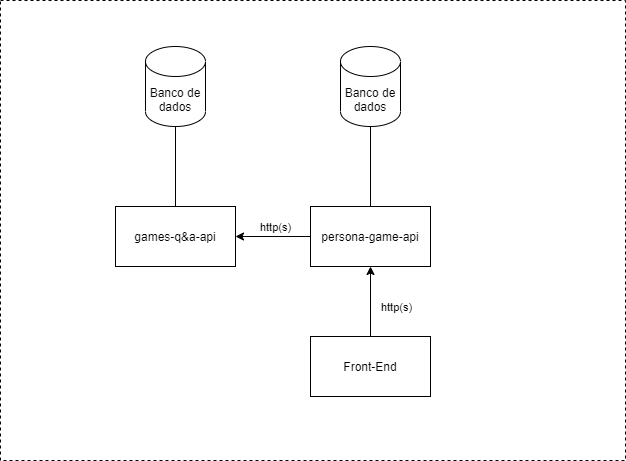
\includegraphics[keepaspectratio=true,scale=0.56]{figuras/arquitetura/diagrama_arquitetura.png}
		\caption{Diagrama Geral de Arquitetura - Fonte: Rossicler Júnior}
	\label{Fig:diagrama_arquitetura.png}
\end{figure}

O primeiro microserviço é o persona-game-api (Figura \ref{Fig:diagrama_arquitetura.png}), ele é composto por uma REST API responsável por se comunicar diretamente com o front-end, fornecendo os dados necessários para o funcionamento do jogo. Este microserviço utiliza de um banco de dados MySQL para armazenamento de dados.

O segundo microserviço é o games-q\&a-api (Figura \ref{Fig:diagrama_arquitetura.png}), ele é composto por uma REST API responsável por fornecer perguntas e respostas a serem usadas no jogo. A decisão de criar um microserviço com apenas esta responsabilidade teve como objetivo melhorar a escalabilidade da criação de outros jogos, podendo utilizar este microserviço como base. Este microserviço utiliza de um banco de dados MySQL para armazenamento de dados.

As comunicações realizadas entre os componentes são realizadas em protocolo HTTP, transmitindo arquivos JSON.

\subsection{Diagrama de Tecnologias}

Como citado na Subseção \ref{ssec:tec_escolhidas}, o jogo utiliza de tecnologias como ReactJS, NodeJS e MySQL. Para uma melhor visualização da comunicação entre essas tecnologias, foi criado um diagrama de tecnologias que representam essas comunicações (Figura \ref{Fig:diagrama_tecnologias.png}).

\begin{figure}[htbp]
	\centering
		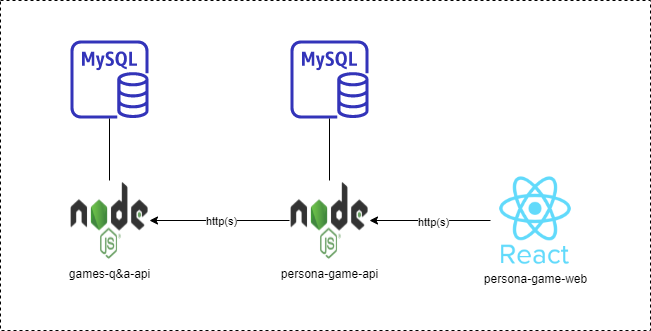
\includegraphics[keepaspectratio=true,scale=0.67]{figuras/arquitetura/diagrama_tecnologias.png}
		\caption{Diagrama de Tecnologias - Fonte: Rossicler Júnior}
	\label{Fig:diagrama_tecnologias.png}
\end{figure}

De acordo com a Figura \ref{Fig:diagrama_tecnologias.png}, a seguir é apresentado uma breve descrição de cada uma dessas tecnologias:

\begin{itemize}
    \item \textbf{\citeauthor{reactjs}} é uma biblioteca de JavaScript front-end para a criação de interfaces, com o foco em páginas web. É uma biblioteca mantida pelo Facebook, Instagram e outros colaboradores.
    \item \textbf{\citeauthor{nodejs}} é um framework de código aberto de JavaScript, com o foco para a criação de back-end. O framework é mantido pela fundação Node.js em parceria com a Linux Foundation.
    \item \textbf{\citeauthor{mysql}} é um sistema gerenciador de banco de dados que utiliza a linguagem SQL como base.
\end{itemize}

\subsection{Visão de Implementação}
\label{ssec:visao_implementacao}

Nesta subseção são apresentados os diagramas de pacotes de cada um dos serviços definidos no Diagrama Geral de Arquitetura (Figura \ref{Fig:diagrama_arquitetura.png}), explicando a responsabilidade de cada módulo/pacote definido.

O diagrama de pacotes é um dos diagramas definidos pela linguagem UML, ele tem como o objetivo a visualização de cada pacote/módulo com suas responsabilidades \cite{guedes2018uml}. Para facilitar a manutenção e evolução do código foi definido uma estrutura na qual cada módulo possui uma responsabilidade bem definida.

Na Figura \ref{Fig:diagrama_pacotes_front.png} é apresentado o diagrama de pacotes referente ao \textit{front-end} do jogo.

\begin{figure}[htbp]
	\centering
		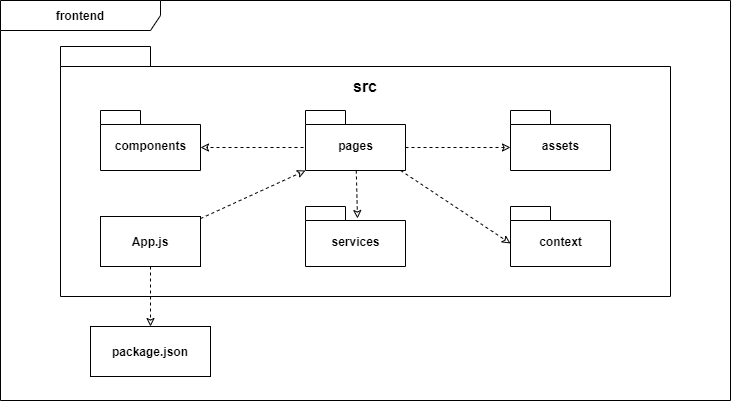
\includegraphics[keepaspectratio=true,scale=0.56]{figuras/arquitetura/diagrama_pacotes_frontend.png}
		\caption{\textcolor{textadded}{Diagrama de Pacotes do Front-end - Fonte: Rossicler Júnior}}
	\label{Fig:diagrama_pacotes_front.png}
\end{figure}

A seguir é listado cada módulo definido na Figura \ref{Fig:diagrama_pacotes_front.png}, com uma breve explicação de cada um:

\begin{itemize}
    \item \textbf{components/} - Possui os componentes utilizados em mais de uma página. Como botões, modals, inputs, etc.
    \item \textbf{pages/} - Contêm todas as páginas da aplicação. As páginas utilizam dos componentes, assets, services e context para o seu funcionamento adequado.
    \item \textbf{assets/} - Possui os arquivos estáticos necessários para a aplicação. Alguns exemplos são imagens, logo, etc.
    \item \textbf{App.js} - Este é o arquivo principal da aplicação, onde inicializa toda a aplicação, chamando todas as páginas a partir das rotas.
    \item \textbf{services/} - Possui os arquivos que realizam todas as requisições necessárias para o funcionamento da aplicação.
    \item \textbf{context/} - Neste módulo são armazenados os arquivos que fazem o uso da Context API fornecida pelo ReactJS, tratando da transferência de dados entre componentes e páginas.
    \item \textbf{package.json} - Este arquivo armazena alguns metadados importantes para o funcionamento da aplicação, como dependências de scripts, versões e etc.
\end{itemize}

Na Figura \ref{Fig:diagrama_pacotes_api.png} é apresentado o diagrama de pacotes referente aos serviços de \textit{back-end} do persona-game-api e games-q\&a-api. Ambos os serviços utilizam desta mesma estrutura, visto que utilizam a mesma tecnologia.

\begin{figure}[htbp]
	\centering
		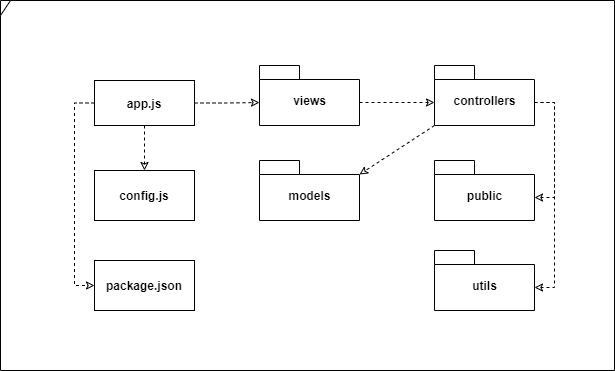
\includegraphics[keepaspectratio=true,scale=0.56]{figuras/arquitetura/diagrama_pacotes_backend.png}
		\caption{\textcolor{textadded}{Diagrama de Pacotes da Persona Game API - Fonte: Rossicler Júnior}}
	\label{Fig:diagrama_pacotes_api.png}
\end{figure}

A seguir é listado cada módulo definido na Figura \ref{Fig:diagrama_pacotes_api.png}, com uma breve explicação de cada um:

\begin{itemize}
    \item \textbf{app.js} - Este é o arquivo principal da aplicação, onde inicializa todo o serviço, chamando as views da API, a conexão com o banco de dados, e etc.
    \item \textbf{views/} - Possui todas as entradas e saídas do serviço, definindo quais endpoints existem, qual método HTTP cada um implementa, e etc.
    \item \textbf{controllers/} - Este módulo é responsável por implementar regras de négocio, fazer a comunicação com o banco de dados, entre outros.
    \item \textbf{config.js} - Este arquivo possui todas as configurações do serviço, como número de porta, secrets, chaves e etc.
    \item \textbf{models/} - Este módulo possui todas as definições de models do banco de dados.
    \item \textbf{public/} - Nesta pasta é armazenado os arquivos públicos, como imagens de usuário, etc.
    \item \textbf{package.json} - Este arquivo armazena alguns metadados importantes para o funcionamento da aplicação, como dependências de scripts, versões e etc.
    \item \textbf{utils/} - É armazenado arquivos com funções de utilidade para o serviço, como funções de formatação, validação de campos, etc.
\end{itemize}

}

% \subsubsection{Especificação do Sistema}

{\color{textadded}
\section{Gerência e Configuração de Software}
\label{sec:gces}

Nesta seção será apresentado o plano de gerência e configuração de software, na qual são definidas as políticas de \textit{issues}, de \textit{branchs}, de \textit{commits}, de \textit{pull request}. Além disso, o plano define como será feito a configuração do ambiente e integração/\textit{deploy} contínuo.

\subsection{Política de Issue}
\label{ssec:politica_issue}

A criação de uma \textit{issue} deve estar ligada a uma nova funcionalidade do software, a correção de um bug ou uma sugestão de melhoria. Ao criar uma nova \textit{issue}, deverá ser selecionado se esta \textit{issue} é uma funcionalidade ou um bug.

Uma issue deve possuir os seguintes campos: um título sucinto para a \textit{issue} e uma descrição da \textit{issue}.

O texto escrito tanto no título quanto na descrição deve estar na língua inglesa, respeitando suas regras de sintaxe e semântica.

\subsection{Política de Branchs}

Para a política de branchs, será utilizado o fluxo definido pelo GitFlow \cite{dwaraki2015gitflow}. Como pode ser visto na Figura \ref{Fig:gitflow.png}, existem algumas regras para a criação de uma nova branch.

\newpage

\begin{figure}[htbp]
	\centering
		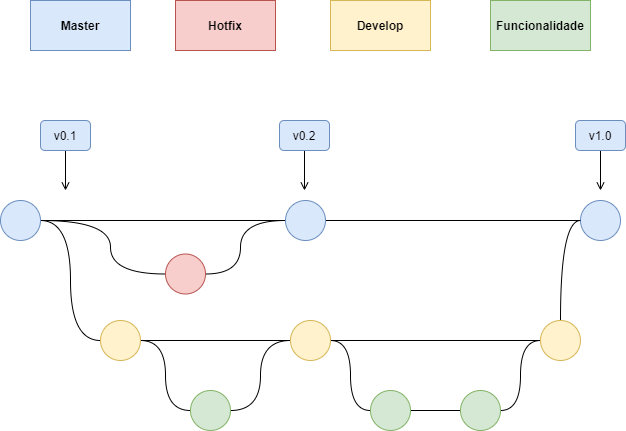
\includegraphics[keepaspectratio=true,scale=0.50]{figuras/gces/git_flow.png}
	\caption{{\color{textadded}GitFlow - Fonte: Rossicler Júnior}}
	\label{Fig:gitflow.png}
\end{figure}

De acordo com a Figura \ref{Fig:gitflow.png}, são listadas algumas das principais regras definidas pelo GitFlow:

\begin{itemize}
    \item Para a criação de uma nova funcionalidade, a \textit{branch} deverá ser criada a partir da develop.
    \item Para a criação de bug (hotfix), deverá ser criada uma branch a partir da master.
\end{itemize}

\subsection{Política de Commits}

Os \textit{commits} devem ser objetivos e atômicos, contendo uma pequena contribuição para resolver certo problema. A mensagem do \textit{commit} deverá descrever brevemente o que foi realizado.

Assim como definido na política de issue (Subseção \ref{ssec:politica_issue}), todo o texto deve ser escrito na língua inglesa.

\subsection{Configuração do Ambiente}
\label{ssec:config_amb}

Para a configuração do ambiente será utilizada uma ferramenta chamada \textit{Docker}. Esta tecnologia fornece uma estrutura para execução de aplicações em \textit{containers} que independem do ambiente que está sendo executado (sistema operacional). A utilização do \textit{Docker} resulta em um desenvolvimento mais fluido, visto que o \textit{Docker} lida com a instalação de todas as dependências do projeto.

Será criado um \textit{Dockerfile} para cada um dos serviços definidos na subseção de Visão de Implementação (Subseção \ref{ssec:visao_implementacao}) contendo toda a configuração necessária para a execução correta de cada um dos serviços.

\subsection{Integração Contínua e Deploy Contínuo}
\label{ssec:ci_cd}

A integração contínua (CI) é uma prática onde o código entregue pelos desenvolvedores passa por uma série de etapas que validam a qualidade do código entregue.

O \textit{deploy} contínuo (CD) é a entrega automatizada de \textit{releases} de um software, em que não é necessário uma ação manual para que novas funcionalidades sejam entregues para a versão oficial do software. Para que esta entrega automatizada seja efetuada, é necessário que primeiro o código passe pela integração contínua (CI). Caso o CI seja realizada com êxito, é feito então o \textit{deploy} das novas funcionalidades aos usuários finais.

Para uma melhor representação das etapas do CI/CD, foi definida uma \textit{pipeline} com as etapas a serem executadas. Para ambos os serviços de back-end e para o front-end, será usado a mesma \textit{pipeline}. Esta \textit{pipeline} é representada na Figura \ref{Fig:pipeline_ci_cd.png}.

\begin{figure}[htbp]
	\centering
		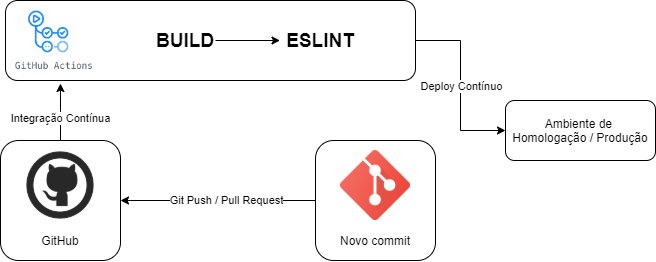
\includegraphics[keepaspectratio=true,scale=0.60]{figuras/gces/integracao_continua.png}
	\caption{{\color{textadded}Pipeline de CI/CD - Fonte: Rossicler Júnior}}
	\label{Fig:pipeline_ci_cd.png}
\end{figure}

}

% - Tecnologias
% - ferramentas

